\documentclass[10pt]{article}
\usepackage[utf8]{inputenc}
\usepackage[T1]{fontenc}
\usepackage{amsmath}
\usepackage{amsfonts}
\usepackage{amssymb}
\usepackage[version=4]{mhchem}
\usepackage{stmaryrd}
\usepackage{graphicx}
\usepackage[export]{adjustbox}
\graphicspath{ {./images/} }
\usepackage{hyperref}
\hypersetup{colorlinks=true, linkcolor=blue, filecolor=magenta, urlcolor=cyan,}
\urlstyle{same}
\usepackage{fixltx2e}

\title{Università degli studi di Catania 
 Corso di laurea triennale in Fisica 
 Esame di Meccanica Analitica Appello del 01.03.2019 }

\author{}
\date{}


\begin{document}
\maketitle
Un sistema materiale, posto in un piano verticale \(\Pi\), é costituito da una sbarra rigida omogenea pesante \(A B\) di massa \(M\) e da un disco omogeneo pesante \(\Gamma\) di massa \(m\), centro \(C\) e raggio \(r\). Il disco \(\Gamma\) é vincolato a rotolare senza strisciare lungo il bordo interno di una guida circolare fissa \(\gamma\) di raggio \(R>r\) e centro \(O\) posta in \(\Pi\). Considerando il riferimento cartesiano ortogonale \(\{O, \vec{x}, \vec{y}\}\), come in figura, l'asta \(A B\), di lunghezza \(L>R\), si muove lungo la direzione verticale \(y\) con l'estremo \(A\) sull'asse \(O y\), mantenendosi ortogonale a questo asse e passando per il centro \(C\) del disco \(\Gamma\). Sul sistema, oltre alla forza peso, agiscono le seguenti forze

\[
\left\{F_{1}=-k(C-Q), C\right\} \quad\left\{F_{2}=-\beta m g \vec{e}_{2}, A\right\} \quad \operatorname{con} \quad k, \beta>0
\]

essendo \(Q\) il punto di intersezione del circolo \(\gamma\) con l'asse delle \(y\) positiva, ed \(\vec{e}_{2}\) il versore dell'asse \(y\).

Il piano II é posto in rotazione uniforme con velocitá angolare \(\underline{w}\) attorno alla verticale \(y\) di \(\Pi\) e tutti i vincoli sono realizzati senza attrito.

Nella ipotesi che la costante elastica \(k=\alpha m g / R\) con \(\beta>\alpha>0\) e scegliendo come coordinata lagrangiana l'angolo \(\vartheta\) che la direzione di \(\overrightarrow{O C}\) forma con la verticale discendente (vedi figura), si chiede di determinare nel riferimento relativo:

\begin{enumerate}
  \item Le configurazioni di equilibrio del sistema, studiandone la stabilitá.

  \item Scrivere le equazioni di moto, determinando gli eventuali integrali primi.

  \item Studiare i moti in prima approssimazione attorno alle configurazioni di equilibrio per il sistema.

\end{enumerate}

\begin{center}
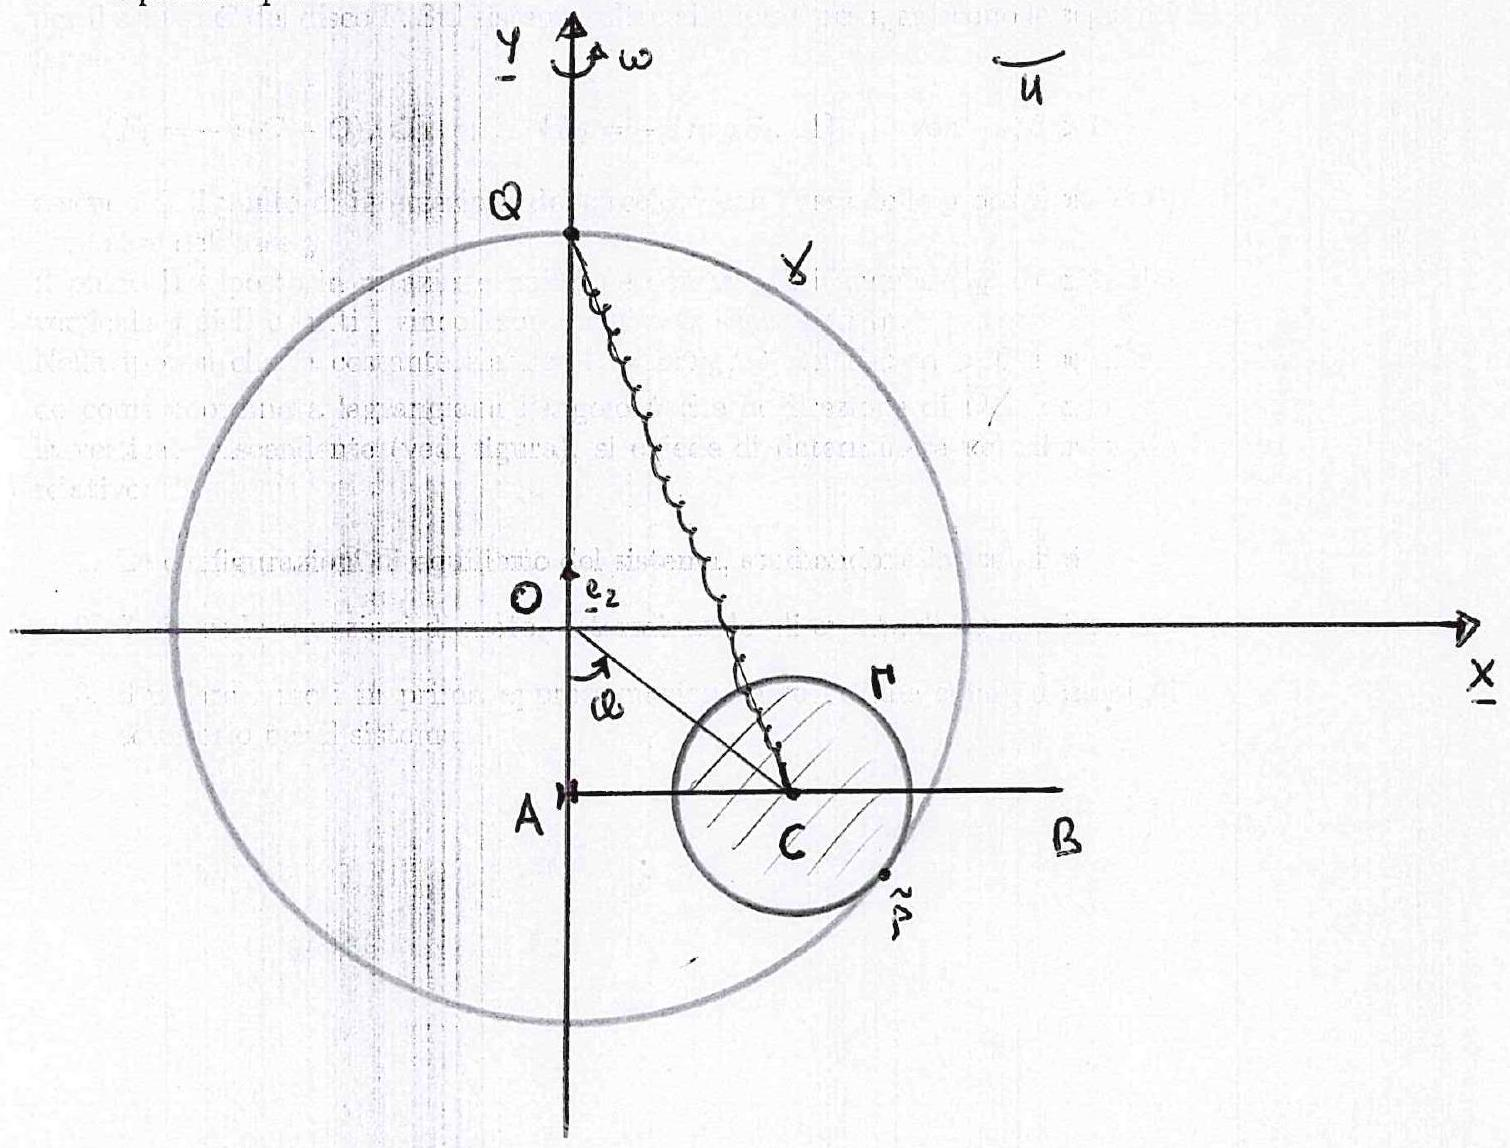
\includegraphics[max width=\textwidth]{2023_04_02_5e0ebfc96e08ff5803bdg-1}
\end{center}

\[
\begin{aligned}
& Q=(0, R) \quad \tilde{P}=(R \sin \theta,-R \operatorname{con} \omega) \\
& A=(0,-(R-r) \cos \theta) \\
& B=(L,-(R-r) \cos \theta) \\
& C=((R-r) \operatorname{sen} \theta,-(R-r) \cos \theta) \\
& \left.F_{1}=-k((R-r) \sin \theta)-R \cos \theta+r \cos \theta-R\right) \quad x \\
& F_{2}=-\beta m g(0,1)
\end{aligned}
\]

\begin{center}
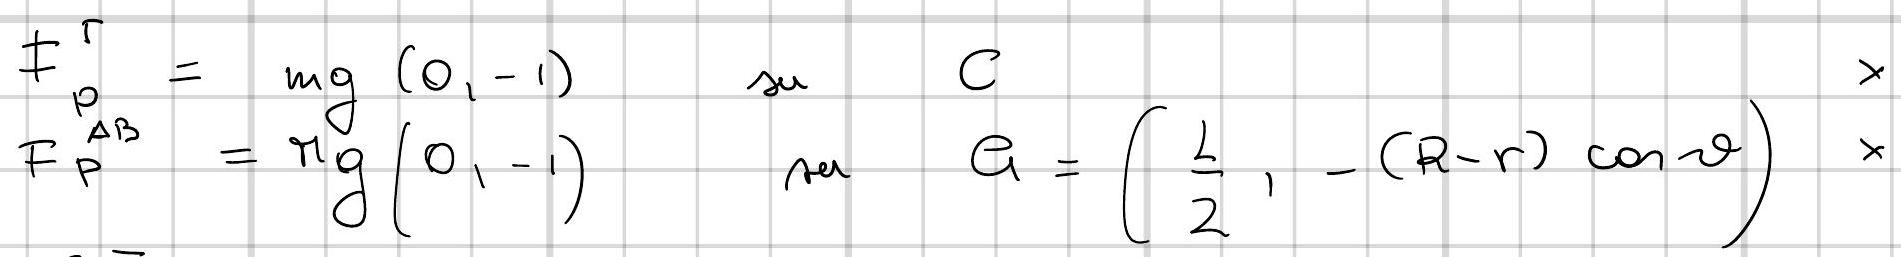
\includegraphics[max width=\textwidth]{2023_04_02_5e0ebfc96e08ff5803bdg-2}
\end{center}

\[
\begin{aligned}
& d F^{c a \bar{~}}=\omega^{2}(P-\bar{P}) \text { dur su ciascun porio } P \text { del siñema } \\
& U_{p}^{\Pi}+U_{p}^{A B}=m g(0,-1) \cdot(c-0)+M g(0,-1) \cdot(G-0)=m g(R-r) \cos \theta+M 0(R-r) \cos \theta=(m+M)(R-r) g \cos \theta \\
& U_{1}=-\frac{1}{2} k(C-Q)^{2}=-\frac{1}{2} k((R-r) \operatorname{sen} \theta,-(R-r) \cos \theta-R)^{2}=-\frac{1}{2} k\left[(R-r)^{2} \operatorname{sen}^{2} \theta+(R-r)^{2} \cos 2 \theta+2 R(R-r) \cos \theta+R{ }^{2}\right]= \\
& =-\alpha \operatorname{cog}(R-r) \cos \theta+\cos \\
& U_{2}=-\beta \operatorname{mg}(0,1) \cdot(A-0)=\beta(R-r) m g \cos \theta \\
& U_{\operatorname{cen}}^{\pi}=\frac{1}{2} \omega^{2} \int_{\Gamma}(p-\bar{p})^{2} d u=\frac{1}{2} I_{y, 0}^{\Gamma} \omega^{2}= \\
& I_{y, 0}=m(C-A)^{2}+\underset{\downarrow}{I_{y, C}^{\Gamma}} \\
& =\frac{1}{2} m(C-A)^{2} \omega^{2}+\cos -= \\
& =\frac{1}{2} m(R-r)^{2} \omega^{2} \operatorname{sen}^{2} \theta
\end{aligned}
\]

\begin{center}
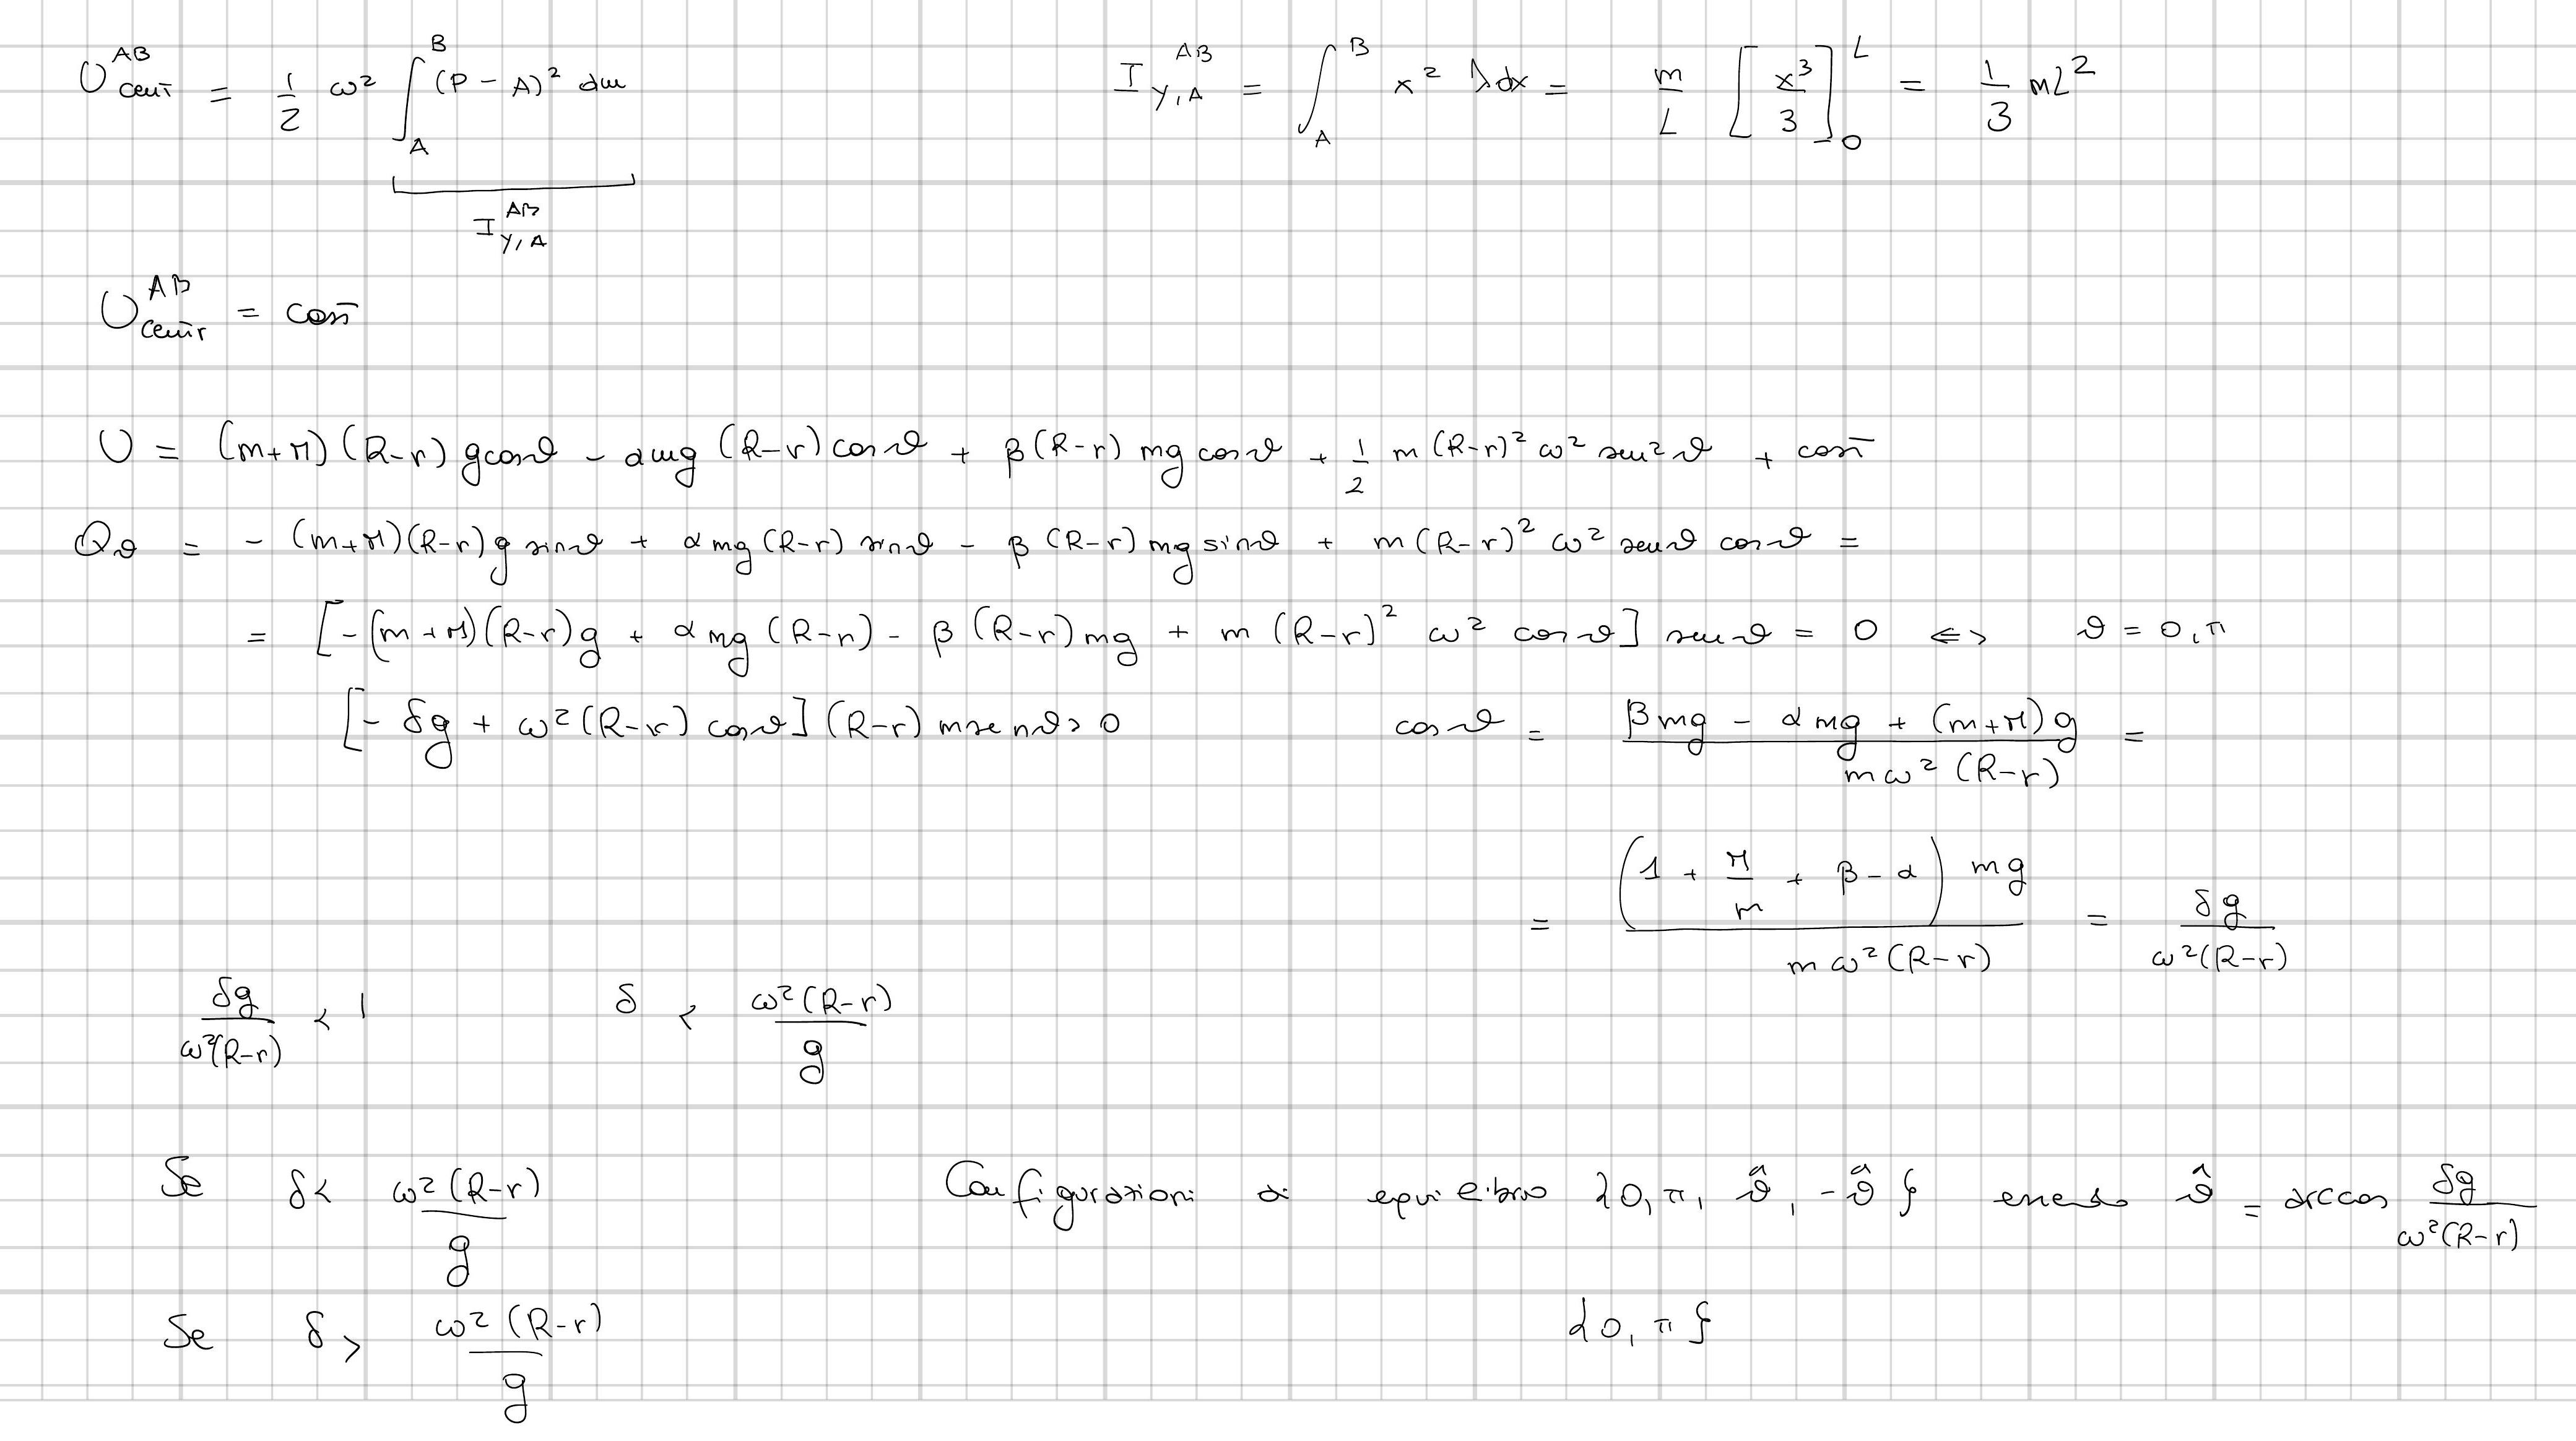
\includegraphics[max width=\textwidth]{2023_04_02_5e0ebfc96e08ff5803bdg-3}
\end{center}

\[
\begin{aligned}
& U_{\theta \theta \theta}=-(m+r)(R-r) g \cos \theta+\alpha m g(R-r) \cos \theta-\beta(R-r) m g \cos \theta+m(R-r)^{2} \omega^{2} \cos 2 \theta \\
& U_{0,}(0)=-(m+M)(R-r) g+\alpha m g(R-r)-\beta(R-r) m g+m(R-r)^{2} \omega^{2}= \\
& =(R-r) m\left[\left(-1-\frac{M}{m}+\alpha-\beta\right) g+(R-r) \omega^{2}\right]=(R-r) m\left[(R-r) \omega^{2}-\delta g\right]>0 \\
& \omega^{2}(R-r)-\delta_{0}^{\pi}>0 \\
& \omega^{2}(R-r)>\delta g
\end{aligned}
\]

\(\vartheta=0\) rtab.le \(x \frac{\delta g}{\omega^{2}(R-r)}>1\), iustabile se \(\frac{\delta g}{\omega^{2}(R-r)}<1\)

Se \(\frac{\delta g}{\omega^{2}(R-r)}=1\)

\[
\begin{aligned}
& {\left[-\delta g+\omega^{2}(R-r) \cos \theta\right](R-r) m \ln \theta>0 \quad[-1+\cos \theta] \omega^{2}(R-r)^{2} m \operatorname{sen} \theta>0<><\varepsilon<2 \pi} \\
& \vartheta=0 \text { i max del poiertiale } \Rightarrow \\
& \Rightarrow \text { eqo eibrio rtabile }
\end{aligned}
\]

\(U_{00}(\pi)=(m+\pi)(R-r) g-\alpha m g(R-r)+\beta(R-r) m g+m(R-r)^{2} \omega^{2}>0 \Rightarrow \pi\) e iusiabile

Deito \(\lambda=\frac{\delta g}{\omega^{2}(R-r)} \quad U_{\theta \theta}(\hat{\vartheta})=U_{v \theta}(-\hat{\vartheta})=m(R-r)^{2} \omega^{2}\left[-\lambda^{2}+2 \lambda^{2}-1\right]=\)

\(=m(R-r)^{2} \omega^{2}\left[\lambda^{2}-1\right]<0 \quad\) percle \(\lambda=\frac{\delta g}{\omega^{2}(R-r)}<1 \Rightarrow \hat{\vartheta} e-\hat{\vartheta}\) stabie.

Energe cinetice

\[
\begin{aligned}
& T^{A B}=\frac{1}{2} M \dot{e}^{2}=\frac{1}{2} M(R-r)^{2} \operatorname{sen}^{2} \theta \dot{\theta}^{2} \\
& T^{\Gamma}=\frac{1}{2} m \dot{C}^{2}+\frac{1}{2} I_{z, c}^{n} \Omega^{2}=\quad I_{z, c}=\iint \rho^{2} d u=\int \rho^{2} \sigma \rho d \rho d a= \\
& =\frac{1}{2} m(R-r)^{2} \dot{\theta}^{2}+\frac{1}{4} m r^{2} \Omega^{2} \quad=\frac{m}{\pi r^{2}} \int_{0}^{r} \rho^{3} d \rho \int_{0}^{2 \pi} d \alpha= \\
& V_{\hat{p}}=0=\dot{C}+\Omega x(\hat{p}-c) \quad=\frac{m}{\pi r^{2}} \frac{r^{4}}{4} \quad 2 \pi=\frac{1}{2} m r^{2} \\
& \left|\begin{array}{ccc}
\hat{\imath} & \hat{\jmath} & \hat{k} \\
0 & 0 & \Omega \\
\text { rame } & - \text { ran } \theta & 0
\end{array}\right| \quad \tilde{P}=(R \sin \theta,-R \cos \theta) \\
& (r \cos \theta \Omega, r \sin \theta \Omega, 0) \quad C=((R-r) \operatorname{sen} \theta,-(R-r) \cos \theta) \\
& \dot{C}=((R-r) \cos \theta \dot{\theta},(R-r) \operatorname{mi\theta } \theta)=(r \cos \theta \Omega, r \sin \theta \Omega, 0) \quad \begin{array}{l}
(R-r) \cos \theta \dot{\theta}=r \cos \theta \Omega \\
(R-r) \min \theta=r \sin \Omega
\end{array}
\end{aligned}
\]

Euerpia ro canderva

\[
\begin{aligned}
& T^{r}=\frac{1}{2} m(R-r)^{2} \dot{\theta}^{2}+\frac{1}{9} m(R-r)^{2} \dot{\theta}^{2}=\frac{3}{4} m(R-r)^{2} \dot{\theta}^{2} \\
& T=\frac{1}{2} M(R-r)^{2} \operatorname{sen}^{2} \theta \dot{\theta}^{2}+\frac{3}{4} m(R-r)^{2} \dot{\theta}^{2} \\
& \frac{\partial T}{\partial \dot{\theta}}=M(R-r)^{2} \operatorname{sen}^{2} \theta \dot{\theta}+\frac{3}{2} m(R-r)^{2} \dot{\theta} \\
& \frac{d}{d t} \frac{\partial T}{\partial \theta}=M(R-r)^{2} m m^{2} \theta \ddot{\theta}+2 \pi(R-r)^{2} \operatorname{sen} \theta \cos \theta \dot{\theta}^{2}+\frac{3}{2} m(R-r)^{2} \theta \\
& \frac{\partial T}{\partial \theta}=M(R-r)^{2} \operatorname{sen} \theta \cos \theta \dot{\theta}^{2}
\end{aligned}
\][

\textbackslash left\href{%5Cnot-r}{\textbackslash frac\{3\}\{2\} m+\textbackslash pi \textbackslash operatorname\{sen\}\^{}\{2\} \textbackslash theta\textbackslash right}\^{}\{2\} \textbackslash ddot\{\textbackslash theta\}+M(B-r)\^{}\{2\} \textbackslash operatorname\{sen\} \textbackslash theta \textbackslash cos \textbackslash theta \textbackslash theta\^{}\{2\}=[-\textbackslash lambda+\textbackslash cos \textbackslash theta] m \textbackslash omega\textsuperscript{\{2\}(R-r)}\{2\} \textbackslash operatorname\{sen\} \textbackslash theta

][

\textbackslash left[\textbackslash frac\{3\}\{2\} m+\textbackslash pi \textbackslash operatorname\{sen\}\^{}\{2\} \textbackslash theta\textbackslash right] \textbackslash ddot\{\textbackslash theta\}+\textbackslash pi \textbackslash operatorname\{sen\} \textbackslash theta \textbackslash cos \textbackslash theta \textbackslash dot\{\textbackslash theta\}\^{}\{2\}=m \textbackslash omega\^{}\{2\} \textbackslash sin \textbackslash theta(\textbackslash cos \textbackslash theta-\textbackslash lambda)
] Madi enearittati

\[
\frac{3}{2} m \ddot{\theta}=\left.Q_{\theta}\right|_{s}+\left.U_{-0}\right|_{s}\left(\theta-\theta_{s}\right)
\]

\(S_{1} \quad \theta=0\)

\[
\begin{aligned}
& \frac{3}{2} m \dot{\theta}=m\left[\omega^{2}-\delta g\right] \theta=\quad m \omega^{2}[1-\lambda] \vartheta \\
& \frac{3}{2} m t^{2}=m \omega^{2}(1-\lambda) \rightarrow \tau^{2}=2 \frac{\omega^{2}(1-\lambda)}{3}>0 \Leftrightarrow \lambda<1
\end{aligned}
\]

\(\lambda<1\) woti iperbolici \(\lambda=1\) woti uniformi \(\rightarrow\) non a sems \(e_{a}\) \(\lambda>1\) wesi arcwonici eluedriftatione

\[
\begin{aligned}
S_{2} \quad \theta=\pi & \frac{3}{2} m \ddot{\theta}- \\
& =m \quad \omega^{2}\left[\frac{\delta g}{\omega^{2}(R-r)^{2}}+1\right](\theta-\pi) \quad \text { Cerco rhmer } \quad \theta-\pi=\theta_{0} e e^{t}
\end{aligned}
\]

\(0<\lambda<1 \quad \tau^{2}=\frac{2}{3} \quad \omega^{2}\left(\frac{\delta g}{\omega^{2}(R-r)^{2}}+1\right) \rightarrow 0 \Rightarrow\) mot iperbale.

\(S_{3} \quad \theta=\hat{\theta}\)

\[
\frac{3}{2} m \ddot{\vartheta}=m \omega^{2}\left[\lambda^{2}-1\right](\theta-\hat{\vartheta}) \quad,-\hat{\vartheta}=\theta_{0} e^{\alpha t}
\]

\[
\frac{3}{2} m \alpha^{2}=m \omega^{2}\left(\lambda^{2}-1\right)
\]

\[
a^{2}=\frac{2}{3} \omega^{2}\left(\lambda^{2}-1\right)<0 \quad \Rightarrow \text { moti drmonici }
\]

Andogle conideradin valyow per \(v=-\hat{\theta}\)


\end{document}